\documentclass[a4paper,11pt]{report}
\usepackage{natbib}

\usepackage[brazil]{babel}
\usepackage[utf8]{inputenc}
%\usepackage[ruled]{algorithm}
%\usepackage[noend]{algorithmic}
\usepackage{amsmath}
\usepackage{amssymb}
\usepackage{amsbsy}
\usepackage{enumerate}
\usepackage{graphicx}
\usepackage{float}
\usepackage{indentfirst}
\usepackage{latexsym}
\usepackage[ruled,vlined]{algorithm2e}
\usepackage{amsthm}
\usepackage{multicol}
\usepackage{verbatim}
\usepackage{color}
\usepackage{tikz}
\usepackage{hyperref}
\hypersetup{
    colorlinks=true,
    linkcolor=black,
    filecolor=magenta,      
    urlcolor=black,
    pdftitle={Algoritmos de Rearranjo de Genomas},
    pdfpagemode=FullScreen,
    }


% Folha A4
\setlength{\parskip}{.2cm}
\setlength{\textwidth}{16.5cm}
\setlength{\textheight}{21.5cm}
\setlength{\topmargin}{0cm}
\setlength{\oddsidemargin}{0cm}
\setlength{\evensidemargin}{0cm}
\setlength{\baselineskip}{4.2cm}

% 'Variáveis globais' (substitua!)
\newcommand{\titulo}{Algoritmos de Rearranjo de Genomas}
\newcommand{\autorA}{Rinaldo Reverte Mendes Junior}
\newcommand{\curso}{Ciência da Computação}
\newcommand{\orient}{Orientador: Prof$^\text{\footnotesize o}$ Fábio Henrique Viduani Martinez}
\newcommand{\corient}{Coorientador: Prof$^\text{\footnotesize o}$ Francisco Elói Soares de Araújo}
\newcommand{\data}{junho de 2021}

% 'Comandos que criados por mim' (substitua!)
\newcommand{\EA}[1]{\textcolor{red}{#1}}
\newcommand{\RR}[1]{\textcolor{green}{#1}}
\newcommand{\FV}[1]{\textcolor{blue}{(Fábio: #1)}}
\newcommand{\dif}{\mbox{\emph{dif}}}
\newtheorem{lema}{Lema}[section]
\newcommand{\reversao}[2]{\Big[{#1}, {#2}\Big]}

\newtheorem{prop}{Propriedade}
\newtheorem{pr}{Proposição}

\def\prova{\noindent \textbf{Prova}. \ignorespaces}
\def\endprova{\vspace*{-.2cm}\hfill $_{\Box}$ \vspace*{5mm}}

\begin{document}

\pagestyle{empty}
\newpage
\input capa.tex

\newpage
\pagestyle{plain}
\pagenumbering{roman}
\setcounter{page}{1}
\input resumo.tex
\newpage
\ \
\newpage
\tableofcontents
\newpage
\pagenumbering{arabic}
\setcounter{page}{1}


\chapter{Introdução}
    
        % O problema de distância editável do qual calcula-se a quantidade miníma de operações (inserção, remoção e substituição) necessárias para transformar uma \textit{string} em outra tem-se mantido em relevância a alguns anos. Uma variação deste problema nos chamou a atenção na área da Biologia mais precisamente no campo de Rearranjo de genomas, este problema é o de distância de ordenação por reversões que consiste em   calcular a menor série de reversões necessárias para transformar uma permutação em outra. 
    
    O problema de Rearranjo de Genomas consiste em calcular a menor quantidade de eventos de rearranjo necessários para transformar um genoma em outro afim de estimar uma distância evolucionária. Estes eventos podem ser provenientes de mutações cromossômicas estruturais, como: transposições, reversões, translocações, entre outras. Para a modelagem do problema utilizamos permutações que descrevem a ordem dos genes nos cromossomos correspondentes, e em relação aos eventos de rearranjo, neste trabalho estudamos um evento em especifico que são as reversões. Nosso foco sempre será encontrar a quantidade miníma de reversões, pois consideramos que a natureza seja parcimoniosa quanto a evolução. Essa pressuposição corresponde à realidade principalmente para distâncias pequenas. Assim nos dedicamos a entender os fundamentos descritos por \cite{kececioglu1995exact} e os algoritmos propostos como solução deste problema: Um algoritmo aproximado (\textit{Greedy}) que utiliza de uma estratégia gulosa que a cada iteração seleciona a melhor solução local e constrói assim os resultados, e um algoritmo exato (\textit{Branch and Bound}) que enumera os candidatos a solução ótima e utiliza de algoritmos que fornecem limitantes para diminuir a quantidade destes candidatos até que só sobre a melhor solução.
    
    % além de reproduzirmos versões dos algoritmos desenvolvidos por ele para a solução deste problema.
    
      Este texto está organizado na seguinte estrutura: De início na Seção \ref{fundamentos}, fornecemos o arcabouço necessário para a modelagem e entendimento do problema e desenvolvimento das soluções. Adiante, na Seção \ref{Algoritmos}, apresentamos os algoritmos aproximado e exato e descrevemos suas implementações e particularidades. Após isso, na Seção \ref{cap:experimentos} apresentaremos experimentos feitos em cenários específicos com permutações geradas, de modo a medir os desempenhos dos algoritmos e trazer um comparativo entre eles. Ao fim, na Seção \ref{cap:conclusao}, temos nossas conclusões e análises finais.
%   Na Biologia Molecular, a medida que o mapeamento e sequenciamento do DNA tornam-se processos de larga escala, um leque de problemas é aberto constantemente para inúmeras áreas de pesquisa, entre elas a Computação. Um destes problemas é o de
  
% A necessidade de se encontrar a quantidade mínima de operações que transformem uma permutação em outra parte do conceito de parcimônia filogenética, onde o conjunto de menor número de transformações possui a maior possibilidade estatística de estar correto (caminho de menor energia) e com isso o conceito de medida usável para distância evolutiva é construído. As operações que usamos para medir a distância evolutiva são variadas: inversões/reversões, transposições, inserções, exclusões, substituições, etc. Todas elas são aplicadas a subcadeias da permutação original. No nosso caso, as operações são restritas a reversões, ou seja, encontrar a menor quantidade de reversões necessárias para transformar uma dada permutação em outra dada permutação. Também podemos estar interessados na sequência de reversões que se refere a essa quantidade mínima de reversões. Dessa forma, estudamos um problema de busca e otimização. 
  
%   (contar a sequencia de passos de kececioglu, o que o nos é garantido)
  
%   mostrar algoritmo exato
  
  %Revisão Bibliográfica, sugestão professor Fábio  



\chapter{Fundamentos}
\label{fundamentos}
Nesta seção, introduzimos definições e conceitos necessários para a compreensão de nossos métodos e soluções. Algumas dessas definições são acompanhadas de exemplos mais práticos e provas de suas propriedades.

\section{Permutações}

% \textcolor{blue}{
% \textbf{Trechos em azul são transcritos de Kececioglu}\\
% \textbf{Permutação}\\
%  Nos problemas matemáticos que consideramos, nos damos a sequência de $n$ genes em 2 organismos mono-cromossômicos relacionados ou 2 organelas, os quais nós representamos por permutações $\sigma = $ $(\sigma_1 \ \sigma_2 \ \ldots \ \sigma_n)$ e $\gamma$ = $(\gamma_1 \ \gamma_2 \ \ldots \ \gamma_n)$. Nesta notação $\sigma_i$ é denotado  $\sigma_(i)$. Estas ordens de genes vem frequentemente de mapeamentos genéticos que são a destilação do trabalho de muitos experimentos geneticistas. Na prática atual, as posições dos genes são cada vez mais encontradas pela comparação de sequências ou hibridização de DNA, oposto aos experimentos de mapeamento da genética tradicional.
%   Nós modelamos um inversão como a reversão de um intervalo de elementos, Formalmente uma reversão de um intervalo $[i, j]$ é a  permutação. (Imagem)
%   Definição: O problema de distância de reversão sobre uma permutação é, dado permutações $\pi$ e $\rho$, encontrar uma serie de reversões $\sigma$ tal que:
%   $ \pi \ \circ \ \sigma_1 \ \circ \ \sigma_2 \ \ldots \ \sigma_d  = \rho$
%   com d mínimo.
%   Nós chamamos d de distância de reversão entre $\pi \ e \ \rho$. Como distância editável, isso satisfaz os axiomas de uma métrica. Distância de reversão mensura uma quantidade de evolução que deve ser tomada  a nível cromossômico, assumindo que a evolução procedeu por inversões. Note que  a distância de reversões entre $\pi$ e $\rho$ é igual a distância de reversão entre $\pi^{-1} \circ \sigma$ e a permutação identidade $\iota$, onde $\pi^{-1}$ denota a inversa de $\pi$. Portanto podemos tomar como entrada $\phi = \pi^{-1}\rho$ e computar sua distância de $\iota$, nós chamamos essa formulação do problema de ordenação por reversões. Note também que o alfabeto de tamanho limitado, como um caso especial resolve o problema de distância de reversões sobre uma permutação.
% }

\textcolor{red}{
% \textbf{Trechos em vermelho estão sendo adaptados.}\\
%  Para o contexto do problema que estudamos, damos a sequência de $n$ genes em 2 organismos mono-cromossômicos relacionados ou 2 organelas, os quais nós representamos por permutações $\sigma = $ $(\sigma_1 \ \sigma_2 \ \ldots \ \sigma_n)$ e $\gamma$ = $(\gamma_1 \ \gamma_2 \ \ldots \ \gamma_n)$. Nesta notação $\sigma_i$ denota  $\sigma_(i)$.
}
Em todas as células vivas, as instruções genéticas hereditárias necessárias para manter um organismo vivo, são armazenadas nos \textit{genes}, os elementos que contêm a informação
que determina as características de uma espécie como um todo, bem como as de um indivíduo. O \textit{gene} é um segmento de uma molécula de DNA (ácido desoxirribonucleico), e cada gene é composto por uma sequência específica de bases nitrogenadas: \textbf{Adenina (A), Citosina(C), Guanina (G), Timina (T)}  que são códigos (instruções) para produzir uma proteína que desempenha uma função específica no organismo \cite{brucealbert}. Em nossos estudos, consideramos a sequência de $n$ genes em dois organismos unicromossomais relacionados, com um mesmo conjunto de genes e cada gene ocorrendo uma única vez em cada genoma. Representamos cada cromossomo por uma \textbf{permutação}, onde cada elemento é um gene. Uma \textit{permutação} $\pi$ sobre um inteiro $n$ é uma função:
\[\pi : \{1,2,\ldots,n\} \rightarrow \{1,2,\ldots,n\}, \]
tal que, para todo $i, j$ como $i \neq j$ temos que $\pi(i) \neq \pi (j)$, o que implica que $\pi$ é bijetora. O $i$-ésimo elemento $\pi(i)$ de $\pi$ também é denotado $\pi_i$, ou seja,
% \FV{Precisa dizer que são bases nitrogenadas que compõem o DNA}
% Cada $\pi_i$ representa o i-ésimo elemento e ocasionalmente será denotado como $\pi(i)$, indicando um gene. Denotamos uma permutação como
\[\pi = ( \pi_1 \ \pi_2 \ \pi_3 \ \ldots \ \pi_n).\]

A \textit{permutação identidade}, denotada por $\iota$, é a permutação $\iota = (1 \ 2 \ 3 \ \ldots \ n)$, ou seja, $\iota_i = i$ para todo~$i$.


\section{Operações com permutações}

Chamamos de $S_n$ o conjunto de todas permutações com $n$ elementos. Uma operação básica sobre permutações em $S$ é a \textbf{composição}, simbolizada por $\circ$, e definida como: dadas duas permutações quaisquer $\pi$ e  $\rho$, temos que $\pi \circ \rho$ (lê-se $\rho$ aplicado a $\pi$) é uma nova permutação que representa os elementos da permutação $\pi$ reordenados em função dos elementos de $\rho$. Mais precisamente, $(\pi \circ \rho)_i = \pi_{\rho_i}$. Consequentemente,

\[\pi \circ \rho = (\pi_{\rho_1} \ \pi_{\rho_2} \ \pi_{\rho_3} \ \ldots \ \pi_{\rho_i}).\]

% Em termos práticos, a composição entre duas permutações reorganiza os elementos de uma permutação utilizando os elementos de outra.

Também definimos o \textbf{elemento neutro} como uma permutação dentre todas à qual sua utilização na composição resulta em nenhuma alteração na permutação original. Existe um único elemento neutro para composição, que é a permutação identidade $\iota = (1, 2, 3 \ldots n)$. Ao aplicarmos $\iota$ sobre um permutação qualquer, ou uma permutação qualquer sobre $\iota$, obtemos sempre a mesma permutação inicial, conforme podemos verificar a seguir. Para qualquer elemento $i$ da permutação identidade $\iota$, temos que: 
    % \[ \iota(i) = i\] 
    % \[\pi \circ \iota = \pi = \iota \circ \pi \]
    % \[ \pi(\iota(i)) = \pi(i) = \iota(\pi(i)). \] 
    
    \[(\iota \circ \pi)_i = \iota_{\pi_i} = \pi_i 
    = \pi_{\iota_i} = (\pi \circ \iota)_i. \]

\subsection{Inversa de uma permutação}


% Como uma permutação é uma função bijetora, ela também admite uma inversa. Dada uma permutação $\pi$ sobre $n$, construímos
Desde que $\pi$ é uma bijeção, sua inversa $\pi^{-1}$ está bem definida: $\pi_i = j \Rightarrow \pi^{-1}_j = i$. 

% E mostramos que $\pi^{-1}$ é a inversa de $\pi$: \[\pi \circ \pi^{-1} = \pi^{-1} \circ \pi = \iota. \]
% Dado que $\pi$ é bijetora, $\pi^{-1}$ está bem definido.
% A inversa de uma permutação $\pi$ qualquer é denotada por $\pi^{-1}$, é a permutação que satisfaz:
\begin{prop}
A composição entre uma permutação $\pi$ qualquer e sua inversa $\pi^{-1}$ é igual a permutação identidade $\iota$,

\end{prop}
\begin{prova}
Sejam $i$ e $j$ inteiros tais que $\pi_i = j$. Por definição $\pi^{-1}_j = i$. Segue que:
\[(\pi \circ \pi^{-1})_j = \pi_{\pi^{-1}_j} = \pi_i = j\] 
\begin{center} e \end{center}
\[(\pi^{-1} \circ \pi)_i = \pi^{-1}_{\pi_i} = \pi^{-1}_j = i.\]
Logo, $\pi^{-1} \circ \pi = \pi \circ \pi^{-1} = \iota$.
    %  \[\pi(i) = j\]
    %  \[\pi^{-1}(j) = i\]
    %  \[\pi^{-1}(\pi(i)) = i\]
    %  \[(\pi^{-1} \circ \pi)(i) = i\]
    %  \[\iota(i) = i\]
    %  \[\pi^{-1} \circ \pi = \iota\]
\end{prova}

Em um exemplo, podemos mostrar que em uma permutação inversa a disposição de seus elementos é referente aos índices das posições da permutação original. Por exemplo, considere as permutações:

  \[ \pi = (2^1 \ 5^2 \ 3^3 \ 7^4 \ 1^5 \ 4^6 \ 6^7)\] 
  \begin{center} e \end{center}
 \[ \pi^{-1} = (5^1 \ 1^2 \ 3^3 \ 6^4 \ 2^5 \ 7^6 \ 4^7).\]
 
 Em $\pi$ os números sobrescritos representam os índices de cada posição dos elementos da permutação. O elemento 2, que antes estava na posição 1 na inversa, tornou-se o elemento 1 na posição 2. Assim sendo, os índices de posição agora são os elementos e os elementos agora são os índices.

% Partindo de uma permutação $\pi$ qualquer, $\pi^{-1}$ é uma permutação que possui os elementos invertidos da permutação $\pi$ com os índices de suas posições, índices se tornam elementos e elementos se tornam índices.


%   \[ \pi = (2^1 \ 5^2 \ 3^3 \ 7^4 \ 1^5 \ 4^6 \ 6^7)\]
%  \[ \pi^{-1} = (5^1 \ 1^2 \ 3^3 \ 6^4 \ 2^5 \ 7^6 \ 4^7)\]
 
%   Os números sobrescritos representam os índices das posição de cada elemento na permutação, isto é, $i^j$ significam $\pi(j) = i$.
 
%  Seja $\pi$ uma permutação sobre $n$. Uma permutação $\sigma$ sobre $n$ é a 
%  \emph{inversa} de $\pi$ se $\pi_i = j \Rightarrow \sigma_j = i$, para todo $i$.
 
%  A inversa $\pi^{-1}$ de uma permutação $\pi$ qualquer é a única que satisfaz  $\pi^{-1} \circ \pi = \iota$. A composição entre uma permutação e sua inversa sempre resultará em uma permutação identidade. Segue a prova:
 
%      \[\pi(i) = j\]
%      \[\pi^{-1}(j) = i\]
%      \[\pi^{-1}(\pi(i)) = i\]
%      \[(\pi^{-1} \circ \pi)(i) = i\]
%      \[\iota(i) = i\]
%      \[\pi^{-1} \circ \pi = \iota\]
     
%  A \emph{inversa} de uma permutação $\pi$ é uma permutação $\pi^{-1}$ que satisfaz  $\rho \circ \pi = \iota$. Vale o seguinte resultado:
%  \begin{pr}
% Seja $\pi$ uma permutação sobre $n$.
% A inversa $\pi^{-1}$ é única e $\pi^{-1} \circ \pi = \pi \circ \pi^{-1}$.
%  \end{pr}
 
%  \begin{prova}
%      Suponha que $\sigma_1$ e $\sigma_2$ são inversas de $\pi$.
%      Seja $k$ um inteiro arbitrário tal que $1 \le k \le n$. Como 
%      $\pi$ é uma permutação sobre $n$, existe um único $j$ tal que 
%      $k = \pi_j$. 
%      Como $\sigma_1$ e $\sigma_2$ são inversas temos que
%      $\sigma_1 (k) = (\sigma_1 (\pi_j)) (k) =  (\sigma_1 \circ \pi) (j) = j$ e similarmente $\sigma_2 (k) = j$ o que implica, desde que $k$ é arbitrário, que $\sigma_1 = \sigma_2$.
%  \end{prova}


\subsection{Outras propriedades da composição}

\paragraph{Associatividade de operações.}
Seja $f: S \times S$, uma função sobre um conjunto $S$ qualquer. Podemos dizer que $f$ é associativa se para todos elementos $x, y, z \in S$ temos que $f(x, f(y, z)) = f(f(x, y), z)$.

% A associatividade é a propriedade de uma operação na qual se pode alterar a precedência de suas execuções sem que haja alteração no resultado.

\begin{prop}
\label{prop2}
    A operação $\circ$ é associativa em $S_n$, onde $n \in \mathbb{N}$ .
\end{prop}

\begin{prova}
    % Seja $n \in \mathbb{N}$. Então,
    Seja $\alpha, \beta, \gamma \in S_n$ e $k \in \mathbb{N}, k \leq n$. Então, 
    \begin{eqnarray*}
     \Big( \alpha \circ  (\beta \circ \gamma) \Big) _k & = & 
     \alpha \Big( (\beta \circ \gamma) _k \Big)\\ & = & 
     \alpha \Big( \beta (\gamma_k) \Big)\\ 
     & = & \Big( \alpha \circ \beta \Big) (\gamma_k) \\
     & = & \Big( (\alpha \circ \beta) \circ \gamma \Big) _k
    \end{eqnarray*}
    Como o resultado vale para um $k$ arbitrário, temos que
    $\alpha \circ  (\beta \circ \gamma) = (\alpha \circ \beta) \circ \gamma$.
\end{prova}

% Podemos ver que os parênteses mais internos indicam a precedência das operações de composição, mas por equivalência pudemos demonstrar que \textbf{a composição é associativa}. Sendo assim para qualquer permutação, a precedência das operações de composição não importa.


\paragraph{Comutatividade de operações.}
Seja $f$ uma operação binária em $S_n$. Afirmamos que $f$ é comutativa se para todos elementos $x, y \in S$ temos que $f(x, y) = f(y, x)$.

% A comutatividade é a propriedade de uma operação na qual se pode modificar a ordem dos elementos sem que haja modificação no resultado. 


A composição em $S_n$ não é comutativa, e isso é demonstrado pelo seguinte contra-exemplo. Se $\pi$ = (2, 1, 3, 4) e $\rho$ = (4, 3, 2, 1), então
\[\pi \circ \rho = (4, 3, 1, 2)\]
\begin{center} $\neq$ \end{center}
\[\rho \circ \pi = (3, 4, 2, 1).\]
% Com isso pudemos provar através deste contra-exemplo que a operação de composição não possui a propriedade comutativa.

\section{Reversões}

% o que é uma reversão - o que é aplicar uma reversão a uma permutação.
% Uma reversão é uma permutação. Sejam  $1 \leq i \leq j \leq n$, a permutação $(1 \ 2 \ 3 \ \ldots \ i-1 \ j \ j-1 \ j-2 \ \ldots \ i \ j+1 \ j+2 \ \ldots \ n)$ é também chamada reversão $[i, j]$. Uma reversão $[i, j$ em uma permutação $\pi$ obtém a permutação $\pi \circ [i, j]$. Portanto, \\
% $\pi \circ [i, j] = \pi_1 \ \pi_2 \ \pi_3 \ \ldots \ \pi_{i-1} \ \pi_j \ \pi_{j-1} \ \pi_{j-2} \ \ldots \ i \ j+1 \ j+2 \ \ldots \ n$

% Uma reversão é uma permutação. Denotaremos uma reversão utilizando a notação de $[i, j]$, onde $i$ e $j$ representam os elementos que estão nas extremidades da strip na composição de reversão. Assim, sendo $1 \leq i \leq j \leq n$, a permutação:

Uma reversão é uma permutação. Ela possui uma inversão de um intervalo de elementos $i, j$, onde $i$ e $j$ representam os elementos que estão nas extremidades de um intervalo de elementos da permutação, logo $1 \leq i \leq j \leq n$. Denotamos essa permutação por $[i, j]$:

% \FV{Não entendi: $[i, j]$ é um intervalo?}

% \RR{corrigido}

\[ [i, j] = (1 \ 2 \ 3 \ \cdots \ i-1 \ 
\boldsymbol{j \ j-1 \ j-2 \ \cdots \ i+1 \ i  }\ j+1 \ j+2 \ \cdots \ n).\]

 Aplicar uma reversão $[i, j]$ a uma permutação $\pi$, é composição $\pi \circ [i,j]$. A composição, $\pi \circ [i, j]$ possui o efeito de mudar a ordem dos elementos de $\pi$. Podemos denotar também a reversão como uma permutação $\rho$ para facilitar a visualização, logo aplicando a reversão $\rho$ sobre $\pi$ tem como resultado a composição:
% é uma reversão $[i, j]$ (pois a reversão é da \textit{strip} de elementos de $i$ a $j$). Uma reversão $[i, j]$ em uma permutação $\pi$ obtém a permutação $\pi \circ [i, j]$. Portanto, \\

\[
\pi \circ [i,j] = (
\pi_1 \ \ 
\pi_2 \ \ \ldots \ \
\pi_{i-1} \ \ 
\underbrace{\pi_{i} \ \ \ldots \ \
\pi_{j-2} \ \ 
\pi_{j-1} \ \ 
\pi_{j}} \ \ 
\pi_{j+1} \ \  \ldots \ \ \pi_n) = \pi \circ \rho
\]

% Intervalo este que pode ser de um único elemento até todos os elementos da permutação. Denotamos um intervalo de elementos $i, j$ por $[i, j]$, onde os elementos dentro do intervalo compõem uma subcadeia da permutação, estes tem suas posições invertidas, e os demais elementos fora do intervalo são mantidos em suas posições.
% Sendo $\rho$ uma permutação qualquer, uma reversão $[i, j]$ em $\rho$ pode ser vista assim:
% \[
% \pi = (
% \pi_1 \ \ 
% \pi_2 \ \ \ldots \ \
% \pi_{i-1} \ \ 
% \underbrace{\pi_{j} \ \ 
% \pi_{j-1} \ \ 
% \pi_{j-2} \ \ \ldots \ \
% \pi_{i}} \ \ 
% \pi_{j+1} \ \  \ldots \ \ \pi_n)
% \] 

% \[
% \pi \circ \rho = (
% \pi_1 \ \ 
% \pi_2 \ \ \ldots \ \
% \pi_{i-1} \ \ 
% \underbrace{\pi_{i} \ \ \ldots \ \
% \pi_{j-2} \ \ 
% \pi_{j-1} \ \ 
% \pi_{j}} \ \ 
% \pi_{j+1} \ \  \ldots \ \ \pi_n)
% \]


% Como exemplo: Dois inteiros $i, j \in \mathbb{N}$, $i \le j$, uma reversão de tamanho $[i, j]$, é a permutação 

% \[(1,\ 2,\ 3,\ 4,\ \mathbf{8,\ 7,\ 6,\ 5,}\ 9,\ 10,\ 11,\ 12,\ 13,\ 14,\ 15,) = [5, 8]\]

% \[(1,\ 2,\ 3,\ 4,\ \mathbf{5,\ 6,\ 7,\ 8,}\ 9,\ 10,\ 11,\ 12,\ 13,\ 14,\ 15) = \rho \circ \alpha\]

% Um exemplo mais visual é apresentado a seguir.

% Uma permutação $\pi$ e uma reversão $\alpha = [2, 4]$. 

% \begin{center}
%  \tikz \draw (0,0) node{1} (1,0) node{4} (2,0) node{3} (3,0) node{2} (4,0) node{5};

\begin{tikzpicture}

\draw (0,0) -- (4,0);
\filldraw [gray] (0,0) circle (5pt) [gray] (1,0) circle (5pt) [gray] (2,0) circle (5pt) [gray] (3,0) circle (5pt) [gray] (4,0) circle (5pt);
\end{tikzpicture}

\tikz \draw (0,0) node{1} (1,0) node{2} (2,0) node{3} (3,0) node{4} (4,0) node{5};


\begin{tikzpicture}

\draw (0,0) -- (4,0);
\filldraw [gray] (0,0) circle (5pt) [gray] (1,0) circle (5pt) [gray] (2,0) circle (5pt) [gray] (3,0) circle (5pt) [gray] (4,0) circle (5pt);


\end{tikzpicture}
% \end{center}

\section{Distância entre duas permutações}

A distância de reversão entre $\pi$ e $\rho$ denotada por $d(\pi,\rho)$ é o menor inteiro $k$ tal que existem permutações $\alpha_1,\ldots,\alpha_k$ tal que $\pi \ \circ \ \alpha_1 \ \circ \ \alpha_2 \ \circ \ \ldots \ \circ \ \alpha_k = \rho$. O problema da \textbf{distância de reversão} é: dadas duas permutações quaisquer $\pi$ e $\rho$, determinar $d(\pi,\rho)$. A distância $d$ é uma métrica \cite{Lages} e medir a distância de reversão entre uma permutação $\pi$ qualquer e $\iota$ é calcular a distância da \textbf{ordenação} de $\pi$, denotada por $d(\pi,\iota) = d(\pi)$.
% Assim a distância entre $\pi$ e $\rho$, $d(\pi, \rho) = k$ onde $k$ denota essa quantidade miníma de reversões. Como distância, $d$  satisfaz os axiomas de métrica provados por , mas neste texto omitimos a demonstração destas propriedades.
% \FV{$d$ é uma função? Ou um número?}
% , ou seja, a quantidade de evolução a nível cromossômico que procede as reversões.
% Seja $\pi$ uma permutação qualquer, tal que:

% \[\pi = (\pi_1 \ \ 
% \pi_2 \ \ 
% \pi_3 \ \ 
% \pi_4 \ \ \ldots \ \ 
% \pi_n) \ \ \]
% \begin{itemize}
%     \item $d(\pi_i, \pi_i) = 0$. \\A distância entre um elemento $\pi_i$ e ele mesmo é sempre 0.
%     \item $Se \ \pi_i \neq \pi_j, \ logo      \ d(\pi_i, \pi_j) > 0$. \\A distância entre quaisquer dois elementos distintos de $\pi$ sempre será maior que 0.
%     \item $d(\pi_i, \pi_j) = d(\pi_j, \pi_i)$.
%     \item $d(\pi_i, \pi_k) \leq d(\pi_i, \pi_j) + d(\pi_j, \pi_k)$.
% \end{itemize}

% \FV{Por que ``lema'' (abaixo)?}
\begin{prop}
Calcular a distância de reversões entre as permutações $\pi$ e $\rho$ é equivalente a calcular a distância de ordenação da permutação $\pi^{-1} \circ \rho$.
\end{prop}
\begin{prova}
% Suponha que encontrar a distância de reversão entre as permutações $\pi$ e $\rho$ é equivalente a encontrar a distância de reversão de $\pi^{-1} \circ \rho$ e a permutação identidade $\iota$. Desta forma, podemos reescrever como, $\tau = \pi^{-1} \circ \rho $ e computar a distância de $\tau$  e $\iota$. Esta formulação do problema de distância passa a ser um problema de \textbf{Ordenação por reversões}, ou seja estamos generalizando o problema de distância de reversões de modo que para toda instância do problema o objetivo seja ordenar a permutação.
Sendo $\alpha_i$ uma reversão $[i, j]$, suponha que $\alpha_1, \alpha_2 \ \ldots,\alpha_k$ é uma sequência de reversões que transforma $\pi$ em $\rho$, ou seja:
\[ \pi \ \circ \ \alpha_1 \ \circ \ \alpha_2 \ \circ \ \ldots \ \circ \ \alpha_k = \rho\]

% Adicionando $\pi^{-1}$ e $\alpha_{k} \circ \alpha_{k-1} \ldots \alpha_1$ aos dois lados da equivalência, temos que: \\

Adicionando $\pi^{-1}$ aos dois lados da equivalência, temos que: \\
% \[\textcolor{blue}{\pi^{-1}} \circ \pi \circ \alpha_1 \circ \ldots\alpha_k \circ \textcolor{blue}{\alpha_{k} \circ \alpha_{k-1} \ldots \alpha_1 = \pi^{-1}} \circ \rho \circ \textcolor{blue}{\alpha_{k} \circ \alpha_{k-1} \ldots \alpha_1}\]


\[ \underbrace{\pi^{-1}} \circ \ \pi \circ \alpha_1 \circ \ldots\alpha_k \circ = \underbrace{\pi^{-1}} \circ \rho \]
\begin{center}
$\downarrow$
\end{center}
\[ \underbrace{\pi^{-1} \circ \pi}_{\iota} \circ \ \alpha_1 \circ \ldots  \alpha_k = \pi^{-1} \circ \rho \]

Adicionando $\alpha_{k} \circ \alpha_{k-1} \ldots \alpha_1$ aos dois lados da equivalência, temos que:

\[ \iota \circ \alpha_1 \circ \ldots\alpha_k \circ \underbrace{\alpha_{k} \circ \alpha_{k-1} \ldots \alpha_1} = \pi^{-1} \circ \rho \circ \underbrace{\alpha_{k} \circ \alpha_{k-1} \ldots \alpha_1}\]



Pela Propriedade \ref{prop2} segue que:\\
\[ \iota \circ \underbrace{\alpha_1 \circ \ldots \underbrace{\alpha_k \circ \alpha_{k}}_{\iota} \circ \alpha_{k-1} \ldots \alpha_1}_{\iota} = \pi^{-1} \circ \rho \circ \underbrace{\alpha_{k} \circ \alpha_{k-1} \ldots \alpha_1}\]

\begin{center}
$\downarrow$
\end{center}

\[ \iota = \pi^{-1} \circ \rho \circ \alpha_{k} \circ \alpha_{k-1} \ldots \alpha_1\]
% \[\pi^{-1} \circ \pi \circ \alpha_1,\alpha_2, \ldots,\alpha_k \alpha_{k} \circ \alpha_{k-1} \ldots \alpha_1 = \iota\]
Logo:
\begin{center}
${\alpha_{k} \circ \alpha_{k-1} \ldots \alpha_1}$ transforma $\pi^{-1} \circ \rho$ em $\iota$
\end{center} 
\end{prova}

Com isso, o problema de distância de reversão passa a ser um problema de \textbf{Ordenação por reversões}, ou seja estamos generalizando o problema de distância de reversões de modo que para toda instância do problema o objetivo seja ordenar a permutação.

% uma das permutações se torne sempre a identidade $\iota$, assim nosso objetivo passa ser o de sempre ordenar a permutação de entrada de modo a alcançar a permutação identidade.

% O impacto disso em nossos experimentos e estudos é que sendo um problema de ordenação, nossa permutação objetivo sempre será a permutação identidade.

\section{\textit{Breakpoints} e adjacências}
%Colocar a notacao de elementos adjacentes

 Um \textbf{\textit{breakpoint}} (BP) de uma permutação $\pi$ é um par de elementos $\pi_i, \pi_{i+1}$, tal que $|\pi_{i+1} - \pi_i| \neq 1$. Quando $|\pi_{i+1} - \pi_i| = 1$, chamamos esse par de \textbf{adjacência}, ou seja $\pi_i$ é adjacente a $\pi_{i+1}$ e denotamos por $\pi_{i+1}$ $\sim$ $\pi_i$. Com o intuito de lidar com \textit{breakpoints} nas extremidades das permutações em nossas implementações os elementos $\pi_0 = 0$ e $\pi_{n+1} = n+1$ são adicionados para destacar os BP formados por elementos nas extremidades da permutação, essa mudança não fere a definição anterior pois não aumenta a quantidade de BP da permutação. Assim, garantimos que os elementos das extremidades da permutação estão na posição correta pois temos um referencial para ordenar os demais elementos internos. A quantidade de \textit{breakpoints} em uma permutação $\pi$ é denotada por $\phi(\pi)$ (lê-se fi de pi) e a diferença da quantidade de \textit{breakpoints} entre uma permutação qualquer $\pi$ e uma reversão $\rho$ aplicada a ela é  denotada por $\Delta \phi(\pi)$ (lê-se delta fi), assim $\Delta \phi(\pi) = \phi(\pi) - \phi (\pi \circ \rho)$. Os valores para  $\Delta \phi(\pi)$ sempre estão entre $-2$ e $2$, pois uma única reversão não pode eliminar ou aumentar mais do que 2 \textit{breakpoints} na permutação.
 
Definimos como \textit{strip} de uma permutação $\pi$ um intervalo de elementos $i, j$, $i \leq j$ tal que os elementos nas posições $(i-1, i)$ e $(j,j+1)$ são BP e que não existam BP nos elementos dentro do intervalo. Sendo assim, todos elementos dentro do intervalo são adjacentes. Além disso, caso esses elementos estejam em ordem crescente, dizemos que essa é uma \textit{strip} crescente (SC). Caso contrário, ela será \textit{strip} decrescente (SD). Os elementos $\pi_0$ e $\pi_{n+1}$ inseridos por nós sempre estarão em uma SC.
% Definimos como \textit{strip}
% crescente (SC) como uma faixa de elementos em ordem crescente na permutação, e definimos como \textit{strip} decrescente uma faixa de elementos em ordem crescente na permutação. Essas duas definições nos servem como base para alguns lemas que veremos mais adiante, e nos ajudam a fundamentar o funcionamento dos algoritmos.

\section{Limitantes}
Nesta seção descreveremos os limitantes inferior e superior para $d(\pi)$, ou seja, os limites do quão boas nossas soluções podem ser,
% , considerando os casos mais favoráveis e os mais desfavoráveis.  .
% Para nosso trabalho, assim como \cite{kececioglu1995exact}, uma parte fundamental é entender como é comportamento das metodologias aplicadas para a obtenção das soluções. Dado isso, esta seção descreve dois pontos que usamos como partida para a construção de nossas soluções, eles estão ligados aos algoritmos usados como 

\subsection{Algoritmo Ingênuo -  Limitante Superior}
\label{algoritmo_ingenuo}
O algoritmo ingênuo é uma das maneiras de se obter um limitante superior para o problema de ordenação por reversões. Os passos do algoritmo ingênuo são: faça uma reversão que coloque o elemento $1$ na primeira posição caso ele já não esteja na primeira posição, após isso faça o mesmo para o elemento $2$, repita este processo até que o elemento $n-1$ fique na $(n-1)$-ésima posição da permutação. No pior dos casos, será necessário fazer $n - 1$ reversões. Assim podemos garantir que qualquer permutação será ordenada em no máximo $n - 1$ reversões, e este é o nosso limitante superior, nenhuma outra solução que gaste mais reversões do que esta nos será relevante, ou seja, $d(\pi) \leq n-1$ para qualquer $\pi \in S_n$.


\subsection{Limitante Inferior}
\label{limitante inferior}
Uma das maneiras de se obter um limitante inferior é pela propriedade de remover BP da uma permutação. Ordenar uma permutação é remover todos BP contidos nela, visto que uma reversão afeta apenas duas extremidades de um intervalo de elementos (\textit{endpoints}), o máximo de BP que conseguimos remover com uma única reversão é dois BP no melhor cenário. Podemos generalizar isso para todos os BP de uma permutação, assim nosso limitante inferior será $(\phi(\pi))/2$. Desta forma nosso limitante traduz-se em ordenar a permutação com uma quantidade de reversões que seja a metade da quantidade de BP na permutação pois supomos que cada reversão remove 2BP, existem outras soluções melhores mas para nossos experimentos esse foi o limitante adotado.


\section{Permutações de Gollan}
% \FV{Que notação é essa: $d(n)$?}
A permutação de Gollan $G_n$ é uma permutação que possui uma propriedade especial: $d(G_n) = n - 1$ \cite{kececioglu1995exact}, isto é, requer $n-1$ reversões para ser ordenada. Somente $G_n$ e $G_n^{-1}$ possuem esta propriedade. Para construir uma permutação de Gollan, utilizamos a seguinte regra: 
% \FV{Definição abaixo em inglês?}
% \RR{DEFINIR d()}
\[G_{n+1} \ = \ \left \{
\begin{array}{cl}
  (1), & n \ \mbox{é zero}; \\
   (G_n(1) \ \ G_n(2) \ \ \ldots \ \ (G_n(n-1) \ \ n+1 \ \ G_n(n)),& n \ \mbox{é  ímpar}; \\
    ( G_n(1) \ \ G_n(2) \ \ \ldots \ \ (G_n(n-2) \ \ n+1 \ \ G_n(n) \ \ G_n(n-1)),& n \ \mbox{é par};
\end{array}
\right.\]

A permutação de Gollan tem importância fundamental em nossos experimentos na Seção \ref{cap:experimentos}, pois dado que $d(\pi) \leq n-1$ para todo $\pi \in S_n.\ G_n$ necessita da maior quantidade de reversões para ser ordenada, sendo este um ponto chave para nossas avaliações de desempenho através dos testes executados.

% A permutação de Gollan tem importância fundamental em nossos experimentos na \textbf{Seção 5}, pois por ser a permutação que necessita da maior quantidade de reversões para ser ordenada, consequentemente ela também é a que exige o maior esforço por parte dos algoritmos e das técnicas implementadas, sendo este um ponto chave para nossas avaliações de desempenho através de testes de estresse.

% \begin{figure}[h]
% \caption{Geração de uma PG}

% \centering % para centralizarmos a figura
% 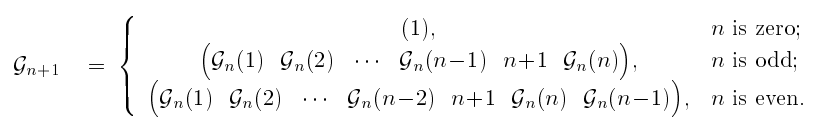
\includegraphics[width=15cm]{Imagens/Gollan.png} % leia abaixo
% \label{figura:Gollan}
% \end{figure}

% \section{Nosso Problema}
% As raízes de nosso problema de distância de reversão vem do problema de \textbf{\textit{edit distance}}, um problema da computação que consiste em 
% encontrar o menor conjunto de operações necessárias para transformar uma \textit{string} em outra.
% \section{Lemas, Teoremas e Corolários}

% \section{Propriedades}

% Algumas propriedades foram extraídas de \cite{kececioglu1995exact} e acompanham nosso processo de compreensão do problema de ordenação por reversões.

% \begin{lema}
% \label{lema1}
%  Toda permutação $\pi$ com uma subcadeia decrescente (SD) possui uma reversão que remove um \textit{breakpoint}.
% \end{lema}
% \begin{prova}
% Seja $x$ o menor elemento em uma subcadeia 
% decrescente em $\pi$ e $i$ o inteiro tal que $\pi_i = x$. Note que $x \ge 1$ pois 0 está em uma subcadeia crescente e $(\pi_i, \pi_{i+1})$ formam um breakpoint. Além disso, $x-1$ está em uma subcadeia crescente. Logo $x-1 \ge 0$ e portanto é um elemento de $\pi$. Seja $j$ o inteiro tal que $\pi_j = x-1$.
% Então, ou $i < j$ ou $i > j$.

% Suponha que $i < j$. Suponha que $(\pi_{j_1}, \pi_j)$ seja um breakpoint, então $(\pi_j, \pi_{j+1})$ é uma adjacência senão $\pi_j$ sozinho seria uma subcadeia decrescente contrariando a minimalidade de $x$. Logo 
% $\pi_{j+1} = x-2$ o que implica novamente que 
% $\pi_j$ está em uma subcadeia decrescente contrariando novamente a escolha de $x$.
% Logo, assumimos que $(\pi_{j-1}, \pi_j)$
% é uma adjacência, ou seja, $\pi_{j-1} = x -2$. Portanto, $(\pi_j, \pi_{j+1})$ é um breakpointo. Logo a reversão $[i,j]$ remove pelo menos um BP.
% \end{prova}

% \FV{O que é ``Lema em passo a passo''?}

% \textbf{Lema em passo a passo:}
% \begin{enumerate}

%     \item $\pi$ possui um SD: escolha o SD aquele que possui o menor elemento $\pi_i$, digamos \[
%     |\ldots  8 \ 7 \ 6 \ 5 |.\]
   
%     \item Todos os números menores que $\pi_i = 5$ estarão em uma SC, pois se não $\pi_i$, não seria o minimal. \[
%     |1 \ 2 \ 3 \ 4 | 8 \ 7 \ 6 \ 5 |.\]
   
%     \item Existe um único \textit{breakpoint} na permutação $\pi$ \[
%     [1 \ 2 \ 3 \underbrace{4 | 8} \ 7 \ 6 \ 5 ].\]
    
%     \item Aplicando uma reversão sobre a SD conseguimos ilustrar que existe uma reversão que remove uma BP
%     \[ [1 \ 2 \ 3 \ 4 \underbrace{8 \ 7 \ 6 \ 5} ].\]
%     \[ [1 \ 2 \ 3 \ 4 \ 5 \ 6 \ 7 \ 8 ].\]

% \end{enumerate}

% \begin{lema}
% \label{lema2}
%  Seja $\pi$ uma permutação com uma SD. Se toda reversão que remove 1 BP de $\pi$ deixa a permutação sem SD, $\pi$ possui uma reversão que remove 2 BP.

% \end{lema}
% \begin{prova}
% Considerando uma SD de $\pi$ contendo o menor elemento $\pi_i$. Portanto a SC que contém $\pi_i-1$ deve estar a esquerda da subcadeia que contém $\pi_i$.
% Considerando a SD de $\pi$ da qual o primeiro elemento, $\pi_j$ é o maior. O elemento $\pi_j+1$ deve estar em uma SC (do contrário $\pi_j$ não é o maior) a direita da subcadeia que contém $\pi_j$
% \end{prova}
% \begin{enumerate}
%      \item $\pi$ possui um SD que possui o menor elemento $\pi_i$, digamos \[
%     \ldots |4 \ 3 \ 2 | \ldots \]
%     \item Portanto a SC que contém $\pi_{i-1}$, deve estar a esquerda da \textit{strip} contendo $\pi_i$ \[
%     \ldots |1 \ 5 \ 6 \ | \ldots | 4 \ 3 \ 2 | \ldots.\]
%     \item $\pi$ possui uma SD que possui o maior elemento $\pi_j$, digamos.
%     \[\ldots |10 \ 8 \ 6 | \ldots \]
%     \item Portanto a SC que contem $\pi_{j+1}$ deve estar a direita da \textit{strip} contendo $\pi_j$
%     \[
%     \ldots |10 \ 8 \ 7 \ | \ldots | 9 \ 11 \ 12 | \ldots.\]
    
    
 
% \end{enumerate}



% \begin{lema}
% \label{lema2}
% Para toda permutação $\pi$, aplicar reversões aleatórias em $\pi$ (ou seja, embaralhar os elementos) aumentará a quantidade de reversões para ordená-la até um determinado ponto.
% \end{lema}

% \begin{prova}
% Seja $\pi_n$ com $n \in \mathbb{N}$, a menor quantidade de BP que $\pi$ pode possuir é 0-BP, ou seja $\pi = \iota$. Reversões aleatórias podem aumentar a quantidade de BP em $\pi$, tirando elementos da posição correta, entretanto o máximo de BP que $\pi$ pode possuir é $(n-1)BP$, a quantidade de BP é limitada pelo próprio tamanho da permutação, ou seja, continuar embaralhando a permutação não aumentará a quantidade de BP, consequentemente a quantidade de reversões necessárias para ordenação também não aumentará. 
% \end{prova}

% aumentar a quantidade miníma necessária de reversões para se ordenar a permutação sem aumentar a quantidade de elementos da permutação só é possível até um determinado ponto.


% \FV{De novo, uma enumeração abaixo}
% \textbf{Lema em passo a passo:}

% \begin{enumerate}
%     \item O mínimo de \textit{breakpoints} que uma permutação sobre $n$ pode ter é 0 BP, ou seja é a permutação identidade.
%     \item O máximo de breakpoints que uma permutação $\pi$ qualquer sobre $n$ pode ter é $n-1$ BP.
%     \item A partir de uma permutação identidade podemos aplicar múltiplos embaralhamentos que aumentem a sua quantidade de BP, consequentemente aumentam a quantidade de reversões necessárias para a ordenação.
%     \item Porém, a quantidade de BP $\phi(\pi)$ é limitada por $n-1$, não sendo possível aumentar essa quantidade apenas embaralhando a permutação, sem modificar o valor de $n$.
%     \item Logo, podemos garantir que há um limite do quanto é possível aumentar a "dificuldade" de se ordenar uma permutação (onde aumentar a dificuldade traduz-se como aumentar a quantidade de reversões necessárias para ordenar) com base em sua quantidade de elementos. Com isso a partir de determinado ponto esta dificuldade torna-se independente da quantidade de embaralhamento aplicado à permutação, 
% \end{enumerate}

 \section{Permutações de teste}

 Além das permutações de Gollan, outras permutações foram utilizadas nos experimentos descritos na Seção~\ref{cap:experimentos}, construídas a partir de um pré-processamento. A primeira classe de permutações criada foi a de permutações aleatórias (PR). Neste caso, iniciamos a partir de permutações identidade de tamanhos variados e utilizamos o método \textit{shuffle}() da biblioteca \textit{random} da linguagem Python. Este método embaralha os elementos da permutação criando assim uma permutação aleatória.  
  \[ \iota = (1 \ 2 \ 3 \ 4  \ \ldots \ n) \rightarrow \textit{shuffle}(\iota) \rightarrow (\pi_1 \ \pi_2 \ \pi_3 \ \ldots \ \pi_n)=\pi \neq \iota.\]
 
 A segunda classe de permutações que criamos são as permutações geradas por reversões aleatórias (PGR), iniciando com uma permutação identidade e escolhendo aleatoriamente dois números inteiros $i, j$ tais que  $1 \leq i \leq j \leq n$, utilizando o método \textit{randint}(). Aplicamos uma reversão $[i, j]$, a qual chamamos de reversão de embaralhamento (o seu oposto seria uma reversão de ordenação). Repetimos esse processo inúmeras vezes, utilizando diferentes valores $i, j$, ao fim temos uma permutação gerada por reversões aleatórias:
 
    % \[\iota = (1 \ 2 \ 3 \ 4  \ \ldots \ n)\]
    \[\iota \ \circ \ [i, j] \ \circ \ [i, j] \ \circ \ [i, j] \ \circ \ldots \ \circ \ [i, j] = \pi\]
    
 A partir dos experimentos com PGRs, fomos capazes de visualizar uma propriedade das permutações:

\begin{prop}
\label{prop4}
Aplicar reversões aleatórias em $\pi$ (ou seja, embaralhar os elementos) aumentará a quantidade de reversões para ordená-la até um determinado ponto.
\end{prop}
\begin{prova}
Seja $\pi_n$ com $n \in \mathbb{N}$, a menor quantidade de BP que $\pi$ pode possuir é 0-BP, ou seja $\pi = \iota$. Reversões aleatórias podem aumentar a quantidade de BP em $\pi$, tirando elementos da posição correta, entretanto o máximo de BP que $\pi$ pode possuir é $(n-1)$BP, a quantidade de BP é limitada pelo próprio tamanho da permutação, ou seja, continuar embaralhando a permutação não aumentará a quantidade de BP, consequentemente a quantidade de reversões necessárias para ordenação também não aumentará. 
\end{prova}
% Cada $\rho_i$ representa a reversão de um intervalo $[i, j]$.

% \FV{Não consigo entender o que você quis dizer acima. Além do mais, o valor de $n$ agora não é mais o comprimento da permutação?}








\chapter{Algoritmos}
\label{Algoritmos}
\section{Algoritmo exato (\textit{Branch and Bound})}

% \textcolor{blue}{
% \textbf{Esta parte transcrevi diretamente do Texto de Kececioglu}\\
%  Na ultima seção nós obtemos um algoritmo que se aproxima do ótimo aplicando uma estratégia gulosa: de todas reversões, selecione uma que remove o máximo de breakpoints. Para obter um algoritmo que alcança o ótimo, nós usamos uma estratégia Branch and Bound: considerar todas reversões, e remover aquelas que não podem levar a uma solução ótima. No algoritmo nós mantemos 3 variáveis globais: $d*$  , um UpperBound dinâmico sobre o valor solução; $r*$, um vetor de reversões que ordena a permutação em $d*$  passos; e $r$, a série de reversões vigente sob consideração. No inicio inicializamos $d*$ e $r*$ com valores obtidos de um algoritmo UpperBound. O algoritmo que nós usamos é essencialmente guloso visando a frente profundidade fixa. 
%   Depois de um obter um Upper Bound no exploramos uma arvore de subproblemas depth-first. Cada invocação do Search corresponde a um nó da árvore e é rotulado com $\pi$, uma permutação para ser ordenada, e $d$, o número de arestas da raiz até o nó. Vetor $r$ é é mantido como uma pilha pelo Search, e trava as reversões sobre o caminho da raiz até o nó atual. Nós escolhemos uma estratégia depth-first para atravessar a árvore com isso usa uma quantidade de polinomial de espaço, mesmo quando a árvore é de tamanho exponencial pois o espaço, não o tempo, é o recurso limitante.
% }

O algoritmo de \textit{Branch and Bound} é um algoritmo exato utilizado para resolver problemas de otimização combinatória. Ele consiste na enumeração passo a passo de todos possíveis candidatos a compor o conjunto solução ótima (em nosso caso, as reversões), explorando todo o espaço de busca e construindo uma árvore de decisão, onde a cada nível abaixo da raiz temos decomposições do problema original. Sendo $\pi$ a raiz da árvore e $\rho_i$ uma reversão representada por uma aresta da árvore, logo $\pi \circ \rho_i$ é um nó filho de $\pi$. Podemos ver uma representação desta árvore na Figura \ref{DecisionTree}. 

% \FV{Usar índices na figura, tais como $\rho_1, \rho_2,$ etc.}

% \begin{figure}[h]

% \centering % para centralizarmos a figura
% 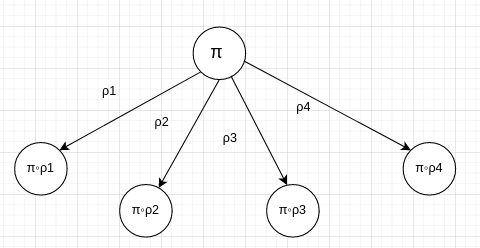
\includegraphics[width=8.0cm]{Imagens/decision_tree.png} % leia abaixo
% \caption{Representação da árvore de decisão do algoritmo exato.}
% \label{figura:Decision Tree}
% \end{figure}

\begin{figure}[h]
    \centering
    \begin{tikzpicture}[level/.style={sibling distance=50mm/#1}]
        \node [circle,draw] (z){$\pi$}
        child {node [circle,draw] (a) {$\pi \circ \rho_1$}
        edge from parent node [above] {$\rho_1$}}
        child {node [circle,draw] (b) {$\pi \circ \rho_2$}
        edge from parent node [above] {$\rho_2$}}
        child {node [circle,draw] (c) {$\pi \circ \rho_3$}
        edge from parent node [above] {$\rho_3$}}
        child {node [circle,draw] (d) {$\pi \circ \rho_4$}
        edge from parent node [above] {$\rho_4$}}
        ;

    \end{tikzpicture}
    \caption{Representação da árvore de decisão do algoritmo exato.}
    \label{DecisionTree}
\end{figure}

Para controlar o tamanho do espaço de busca da solução ótima, dois algoritmos são necessários, para computar os limitantes (\textit{Bounds}): o \textit{UpperBound}() e o \textit{LowerBound}(). Esses algoritmos calculam os valores que podem ser vistos como o intervalo onde a solução ótima se encontra e quanto mais refinados forem, menor será o tempo para processar a solução ótima. Diminuir o espaço de busca através destes algoritmos reflete na árvore de decisão como operações de poda, que diminuem a quantidade de nós, descartando conjuntos de soluções ruins até que apenas a solução ótima reste. Em nível de implementação, o algoritmo constrói uma lista com todas as reversões possíveis de uma permutação $\pi$ e as ordena em ordem decrescente em relação ao número de BPs removidos por cada reversão. Essa lista é percorrida e cada reversão $\rho_i$ é selecionada e aplicada sobre $\pi$. A quantidade de passos, isto é, a distância de um nó da árvore de decisão para a raiz, é incrementada em uma unidade e analisamos se o candidato $\rho_i$ selecionado está dentro dos limitantes correntes; caso esteja, uma chamada recursiva é realizada com $\pi \circ \rho_i$, no lugar de $\pi$; caso contrário, $\pi \circ \rho_i$ e todos os seus filhos na árvore são descartados. São usadas três variáveis globais que são mantidas em nosso algoritmo: um \textit{upperbound} dinâmico $d*$ contendo a quantidade de reversões de nossa solução, uma lista de reversões $r*$ que ordena a permutação em $d*$ passos e uma segunda lista de reversões $r$ com o conjunto de reversões atual sob análise.

Os limitantes são a chave do algoritmo exato, pois um limitante ruim ocasionaria em um aumento grande na quantidade de candidatos a serem analisados. Tendo isso em vista, os métodos escolhidos que calculam os limitantes, apesar de não serem os mais eficientes, são os mais intuitivos com um desempenho aceitável para a nossa proposta. O método para o cálculo do limitante superior que usamos é a maneira mais simples de gerar uma solução para nosso problema, descrita no algoritmo ingênuo na seção \ref{algoritmo_ingenuo}, que garante que nenhuma da sequências de reversões que forem encontradas posteriormente no algoritmo que realizam uma quantidade de passos superior seja considerada. Atualmente, nosso algoritmo que calcula o limitante superior é executado em tempo $\mathcal{O}{(n)}$. Para melhor conveniência, chamaremos o algoritmo ingênuo de \textit{Reversal Sort} e a figura \ref{figura:Execução do Reversal Sort} apresenta alguns passos de sua execução.


\begin{figure}[h]
% \caption{Exemplo \FV{Esta figura não é referenciada no texto e a legenda não diz nada.}}
% \RR{Corrigido}
\centering % para centralizarmos a figura
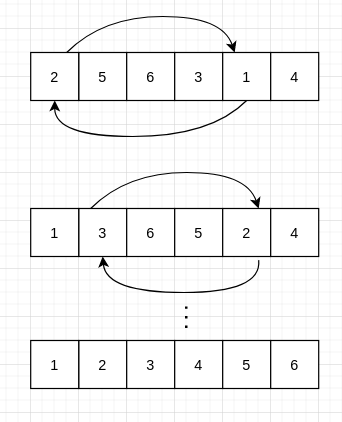
\includegraphics[width=5.8cm]{Imagens/reversalSort.png} % leia abaixo
\caption{Representação da execução do Reversal Sort.}
\label{figura:Execução do Reversal Sort}
\end{figure}


Em relação ao método que calcula o limitante inferior, sua função é devolver um valor para o melhor caso de execução possível, servindo como parâmetro de poda na árvore de decisão a cada iteração da lista de candidatos, ou seja, é calculado dinamicamente. Esse algoritmo é construído a partir da observação de que o melhor cenário é remover dois BPs com uma única reversão, como visto na seção \ref{limitante inferior}. A quantidade de passos de execução é a metade da quantidade de BPs, ou seja $\phi(\pi)/2$. Podemos calcular este limitante em tempo $\mathcal{O}{(n)}$, que é necessário para contar os BPs da permutação.  

A seguir é mostrado um pseudocódigo de nosso algoritmo \textit{Branch and Bound}.

\begin{comment}
A primeiro momento, uma permutação qualquer é dada como entrada na função UpperBound (limitante superior) que garantirá que nossa solução final não seja pior que a encontrada por este limitante. Com isso, as variáveis globais são atualizadas com o conjunto solução (quantidade de passos, e conjunto de reversões ),  encontrado pelo UpperBound, que poderá ser substituído caso encontremos uma solução melhor no processamento principal (função Branch and Bound). Na função principal do algoritmo recebemos a permutação de entrada junto com um 0 referente a quantidade de passos realizados até a solução final, após isso é verificado se a permutação de entrada já esta ordenada (se sim, não há nada a se fazer), e caso não esteja o algoritmo irá iterar em uma lista de reversões de ordem decrescente de $\Delta(\phi)$, a cada iteração a quantidade de passos é incrementada em 1 e a reversão atual é aplicada sobre a permutação. Se a quantidade de passos somada a um LowerBound (limitante inferior, que nos garante que a solução final não será melhor do que a encontrada pelo limitante) for menor que a quantidade passos obtida pelo UpperBound, nós iremos armazenar a reversão feita no conjunto solução e chamaremos a função principal recursivamente, agora com os parâmetros atualizados. Este processo principal é repetido até que a permutação esteja ordenada.
A saída do algoritmo é o conjunto solução contendo a quantidade de passos realizada pela solução ótima assim como as reversões que a compõem.
A seguir será demonstrado um pseudocódigo contendo o Algoritmo Branch and Bound proposto por e o pseudocódigo de nossa implementação do problema seguindo os parâmetros definidos pelo autor no artigo.\\
\end{comment}

\begin{algorithm}[H]
\label{Algoritmo Exato}
\SetAlgoLined
\textbf{Global: d*, r*[1..n], r[1..n]}\;
\textbf{\textit{Branch and Bound}($\pi$)}\;
  \quad  $d*, r*$ = \textbf{\textit{UpperBound}($\pi$)}\;
  \quad \textbf{Search($\pi$, $0$)}\;
  \quad \textbf{return $d*, r*$}\;
\textbf{Search($\pi$, $d$)}\; 
    \quad\If{$\pi$ é a identidade}{
    \quad \quad $d', r' = d, r$\;
    }
\quad \Else{
\For{ cada reversão $\rho$ em ordem decrescente de $\Delta\phi$}{
    \quad $d'$, $\pi'  = d + 1$, $\pi$ $\circ$ $\rho$\;
    \quad \If{$d'$ + \textbf{\textit{LowerBound}($\pi'$)} $<$ $d*$}{
        \quad \quad $r[d'] = \rho$\;
        \quad \quad \textbf{Search($\pi', d'$)}\;
    }
}
} 

\textbf{\textit{LowerBound}($\pi$)}\;
\quad \textbf{return $\lceil$ $\phi(\pi)/ 2$ $\rceil$}\;

\textbf{UpperBound($\pi$)}\;
\quad global $d*, r*$\;
\quad $d*, r* = $ \textbf{ReversalSort($\pi$)}

 \caption{Algoritmo Exato}
\end{algorithm}

% \FV{Esse algoritmo não é referenciado no texto, com um comando \textbackslash\!ref\{\}.}
% \RR{Corrigido}

\section{Algoritmo guloso (\textit{Greedy})}

% O Greedy Algorithm é um algoritmo de aproximação que utiliza uma estratégia gulosa. Algoritmos de aproximação são algoritmos que podem entregar uma solução próxima da ótima, ou seja, são como uma garantia do quão próximo estou de uma solução ótima.

O método guloso é um paradigma de construção de algoritmos que pode ser usado para resolução de problemas de otimização combinatória, consumindo tempo polinomial nos tamanhos de suas entradas, produzindo algoritmos intuitivos. Algoritmos gulosos buscam a cada iteração o melhor candidato local, ou seja, a opção que oferece o benefício mais óbvio e imediato para o problema, assim construindo uma solução passo a passo com cada candidato. Em nosso caso, a solução a ser construída é a menor quantidade de reversões necessárias para ordenar uma permutação. No primeiro momento, a solução mais intuitiva seria a de colocar cada elemento da permutação, um por um, em sua devida posição, executando $n-1$ passos no pior caso para uma permutação de $n$ elementos, como visto na seção \ref{algoritmo_ingenuo}. Porém, esta seria uma solução fraca, pois para alguns casos ela entrega uma resposta muito ruim. Um exemplo é a permutação $(0, n, n-1, \ldots , 2, 1, n+1)$ que poderia ser ordenada com uma única reversão, mas o algoritmo ingênuo usa $n-1$ reversões. A partir da definição de BP, uma solução melhor foi proposta por \cite{kececioglu1995exact}, na qual a cada iteração a reversão que remove o máximo de BPs possível é executada, e em casos de empate opta-se preferencialmente por aquelas que resultam em uma SD. 
% \FV{Usar rótulos e referências (comandos label e ref)}
% \FV{SD foi definido antes?} 
% \FV{O que é?}
% \FV{O que é uma ``resposta não satisfatória''?}

O algoritmo executa enquanto houver BP na permutação e a cada iteração ele busca uma reversão que remova o máximo de BPs possíveis. Nesta busca consideramos três casos, dois deles removem BPs e um caso que não remove nenhum mas ajusta a permutação. O primeiro caso é o  melhor cenário, remover dois BPs com uma única reversão. Caso não seja possível, o algoritmo busca uma reversão que remova apenas um BP com preferência em reversões em que seja deixada uma SD após a reversão. Esta informação adicional de utilizar \textit{strips} para construir uma solução é fruto de lemas e provas elaborados por \cite{kececioglu1995exact}, de onde extraímos dois principais resultados, sendo um teorema e um corolário:

\newtheorem{Theorem}{Teorema}
\begin{Theorem}
\label{teorema}
O algoritmo Greedy ordena todas permutações $\pi$ em no máximo $\phi(\pi)$ passos.
\end{Theorem}
\begin{prova}
Se $\pi$ possui uma SD, o algoritmo Guloso ordena $\pi$ em no máximo $\phi(\pi)$ reversões. Se $\pi$ não possui SD, qualquer reversão escolhida pelo \textit{Greedy} transformar $\pi$ em uma permutação $\pi'$ com SD tal que $\phi(\pi') \leq \phi(\pi)$. \textit{Greedy} ordena $\pi'$ em no máximo $\phi(\pi') - 1$ reversões, e que ordena $\pi$ em no máximo de $\phi(\pi)$ reversões.
Uma vez que $\phi(\pi) \leq n + 1$, \ref{teorema} implica que o algoritmo \textit{Greedy} finaliza em $\mathcal{O}(n)$ iterações e roda em tempo polinomial. Um algoritmo para problemas de otimização que roda em tempo polinomial e entrega uma solução cujo valor esta dentro de um fator $\varepsilon$ conhecido como algoritmo $\varepsilon-$aproximado por ordenação por reversões.
\end{prova}

\newtheorem{Corollary}{Corolário}
\begin{Corollary}
O algoritmo Greedy é uma 2-aproximação para ordenação por reversões.
\end{Corollary}
\begin{prova}
Escreva $Opt(\pi)$ como sendo o mínimo número de reversões para ordenar uma permutação $\pi$, e \textit{Greedy}$(\pi)$ para o número obtido pelo algoritmo \textit{Greedy}. Uma vez que a solução deve remover todos os BPs e qualquer reversão pode remover no máximo dois BPS, temos que
\[ Opt(\pi) \ \ge \ \frac{1}{2}\phi(\pi) \ \ge \ \frac{1}{2}\textit{Greedy}(\pi).\] \\

Ou seja, temos a garantia de que no pior caso não executaremos mais que o dobro do numero de reversões da solução $Opt$.
\end{prova}

% Ou seja, a solução $Opt$ pode ser até duas vezes menor que a quantidade de BP ou que a resposta do algoritmo Greedy. 

O algoritmo \textit{Greedy} beneficia-se deles pois aumenta a garantia de que teremos êxito na remoção de um BP não só no passo atual como também em um passo futuro. Não sendo possível remover um BP que deixa uma SD, faremos apenas a remoção de um BP, mas se nenhum dos casos anteriores forem possíveis de serem executados, um passo de ajuste que não remove BP algum é executado e reorganiza a permutação, abrindo caminho para reversões que removem BPs. Em nenhum momento podemos executar uma reversão que aumenta a quantidade de BPs, pois uma reversão como essa nunca fará parte da solução com menor quantidade de reversões. Isso comprometeria os resultados do algoritmo, além de tornar o laço externo um \textit{loop} infinito. A saída do algoritmo consiste na quantidade de reversões aplicadas na permutação original até alcançar a identidade, além do conjunto de reversões aplicadas, nosso algoritmo \textit{Greedy} possui complexidade de $\mathcal{O}(n^2)$.

A seguir é mostrado um pseudocódigo de nosso Algoritmo \textit{Greedy}.


\begin{algorithm}[H]
\label{Algoritmo Greedy}
\SetAlgoLined
\textbf{Greedy($\pi$)}\;
 $i = 0$\;
 \While{$\pi$ contém BP}{
  $i = i + 1$\;
  Faça uma reversão $\rho$ em $\pi$ que remova o máximo de BP. Se o máximo for 1, priorize reversões que deixam uma sub-cadeia decrescente\;
  $\pi$ = $\pi \circ \rho$\;
 }
 \textbf{return} $i \  \rho_1, \rho_2, \rho_3 ...$\;
 \caption{Algoritmo \textit{Greedy}}
\end{algorithm}

% Alguns Lemas acompanham o desenvolvimento de nosso algoritmo Greedy, e nos são fundamentais para garantir 
% \begin{lema}
% \label{lema3}
% O algoritmo Greedy ordena uma permutação $\pi$ com uma SD em no máximo $\phi(\pi)-1$ reversões.
% %   \textcolor{red}{To Do}
% \end{lema}
% \begin{prova}
% A prova é por indução sobre $\phi(\pi)$. Se $\pi$ possui uma SD, $\phi(\pi)$ $\ge$ 2. Quando $\phi(\pi) = 2$, $\pi$ possui uma única reversão $\rho$ que remove os 2 BP e ordena $\pi$, assim  o \textit{Greedy} irá escolhe-lá.

% Suponha que o lema seja válido para todas permutações $\pi'$ com menos de que $\phi(\pi)$ BP. Desde que $\pi$ possua uma SD, por \ref{lema1} há uma reversão $\rho$ que remove ao menos um BP. Assim o primeiro passo do Greedy transformará uma permutação $\pi$ em $\pi'$ com no máximo $\phi(\pi) - 1$ BP. Se $\pi'$ possui uma SD, Greedy ordenará em no máximo $\phi(\pi) - 2$ por hipótese de indução na qual $\pi$ é ordenado em no máximo $\phi(\pi) - 1$ reversões.
%  Agora consideramos que $\pi'$ não possua SD. Nós argumentamos que $\phi(\pi') = \phi(pi) - 2$. Por suposição $\phi(\pi') = \phi(pi)-1$, a uma única outra possibilidade. Desde que o \textit{Greedy} escolhe a reverwsão que remove o máximo de BP, não deve haver reversão que remova dois BP. Em outras palavras, toda reversão que remover um BP, remove unicamente um BP. 

% \FV{Finalizar a prova}
% \end{prova}

% \begin{lema}
% \label{lema3}
% O algoritmo Greedy ordena uma permutação $\pi$ com uma SD em no máximo $\phi(\pi)-1$ reversões.
% %   \textcolor{red}{To Do}
% \end{lema}
% \begin{prova}
% A prova é por indução sobre $\phi(\pi)$. Se $\pi$ possui uma SD, $\phi(\pi)$ $\ge$ 2. Quando $\phi(\pi) = 2$, $\pi$ possui uma única reversão $\rho$ que remove os 2 BP e ordena $\pi$, assim  o \textit{Greedy} irá escolhe-lá.

% Suponha que o lema seja válido para todas permutações $\pi'$ com menos de que $\phi(\pi)$. Desde que $\pi$ possua uma SD, por \ref{lema1} há uma reversão que remove ao menos um BP. Assim o primeiro passo do Greedy transformará uma permutação $\pi$ em $\pi'$ com no máximo $\phi(\pi) - 1$ BP. Se $\pi'$ possui uma SD Greedy ordenará em no máximo $\phi(\pi) - 2$ por hipótese de indução que ordena $\pi$ em no máximo 1 reversão.

% % \FV{Finalizar a prova}
% \end{prova}

% \newtheorem{Theorem}{Teorema}
% \begin{Theorem}
% O algoritmo Greedy ordena toda permutação $\pi$ em no máximo $\phi(\pi)$ passos.
%   \textcolor{red}{To Do}
% \end{Theorem}
% \begin{prova}
% Se $\pi$ possui uma SD, pelo \ref{lema3}, o algoritmo Guloso ordena $\pi$ em no máximo $\ $
% \end{prova}

% \newtheorem{Corollary}{Corolário}
% \begin{Corollary}
% O algoritmo Greedy é uma 2-aproximação para ordenação por reversões.
% \end{Corollary}
% \begin{prova}
% Escreva $Opt(\pi)$ como sendo o mínimo número de reversões para ordenar uma permutação $\pi$, e \textit{Greedy}$(\pi)$ para o número obtido pelo algoritmo \textit{Greedy}. Uma vez que a solução deve remover todos os BPs e uma reversão remove no máximo dois BPS, temos que
% \[ Opt(\pi) \ \ge \ \frac{1}{2} \ \ge \ \frac{1}{2}\textit{Greedy}(\pi).\]
% \end{prova}

\begin{comment}
\begin{algorithm}[H]
\SetAlgoLined
\textbf{Algoritmo \textit{Greedy}($\pi$)}\;
 i  = 0\;
 \While{$\pi$ contém BP}{
  i = i + 1\;
  \While{1 até n}{
  Procure uma 2-reversao}
\While{1 até n}{
  Procure uma 1-reversao-SD}
 \While{1 até n}{
 Procure uma 1-reversao}
  \While{1 até n}{
 Procure uma 0-reversao}
$\rho = n$-reversao\;
  $\pi$ = $\pi \circ \rho$\;
 }
 \textbf{return} $i \  \rho_1, \rho_2, \rho_3 ...$.\;
 \caption{Algoritmo aproximado}
\end{algorithm}
\end{comment}

% O consumo de tempo deste algoritmo é o seguinte. Observe que o laço principal (mais externo) consome tempo $\mathcal{O}{(\phi(\pi))}$ no pior caso e cada passo interno consumo tempo $\mathcal{O}{(n)}$. Como um todo, o consumo de tempo pode ser simplificado para $\mathcal{O}{(n^{2})}$ e o espaço consumido é $\mathcal{O}{(n)}$. Um algoritmo aproximado se fez necessário nos estudos de \cite{kececioglu1995exact}, pois o \textit{Branch and Bound} possui a amplitude de testes limitada por seu consumo excessivo de tempo. Apesar de não devolver a resposta exata, o algoritmo \textit{Greedy} tem melhor desempenho para permutações extensas, devolvendo um resultado satisfatório em um tempo de execução mais aceitável. 
\begin{chapter}{Experimentos} \label{cap:experimentos}

Com o intuito de analisar os algoritmos da seção anterior, especialmente tempos de execução e médias das quantidades de reversões para obter uma solução, criamos testes utilizando dados simulados, divididos em três categorias. A primeira categoria usa como entrada permutações aleatórias (PR), permutações do tipo identidade embaralhadas uma única vez. Nestes testes, nosso esforço está voltado em observar o tempo de execução e a quantidade média de reversões necessárias para ordenar a instância do problema. A segunda categoria dos testes é utilizando permutações geradas a partir de reversões aleatórias (PGR), que são permutações também construídas a partir da permutação identidade, porém com múltiplos embaralhamentos, sendo nosso foco observar o comportamento dos resultados dos algoritmos em função da quantidade de embaralhamentos. Por fim, a terceira categoria de testes é composta por permutações de Gollan (PG) que, por suas propriedades especiais, necessitam de mais iterações dos algoritmos, sendo o foco da análise do tempo de execução em função do tamanho da permutação. Para maior precisão de nossas análises, os dados utilizados nos experimentos foram construídos a partir da média dos resultados de vários testes, com o intuito de diminuir ruídos na apresentação dos resultados. 
    
Os experimentos foram realizados em uma máquina com as seguintes especificações: processador Intel Dual Core 3,5 Ghz, 8 Gb de memória, sistema operacional Manjaro Linux e linguagem de programação Python3. 

\section{Experimentos com algoritmo \textit{Branch and Bound}}

\subsection{Permutações de Gollan}

No primeiro de nossos experimentos geramos PGs com tamanhos de 6 até 14 elementos, mantendo esse intervalo com o intuito de não ultrapassar o limite de 30 minutos estipulado para resolução de cada permutação. Especificamente neste conjunto de testes optamos por não executar múltiplas instâncias, ou seja, gerar várias PGs e calcular uma média dos resultados, por alguns motivos: o desempenho do algoritmo BnB não é bom e pelo fato do esforço computacional necessário para se ordenar uma permutação de Gollan ser alto. Note que na figura \ref{Grafico1}, a curva se mantém modesta inicialmente e a partir de um determinado ponto (tamanho da permutação $\ge 14$) apresenta uma explosão, crescendo rapidamente. Por este comportamento visto no gráfico podemos pressupor que estendendo esse gráfico para PGs com mais elementos, essa curva se assemelharia cada vez mais a de uma função exponencial, que é condizente com a complexidade do algoritmo BnB.

\begin{figure}[H]
\centering
  \begin{minipage}[b]{0.5\textwidth}
    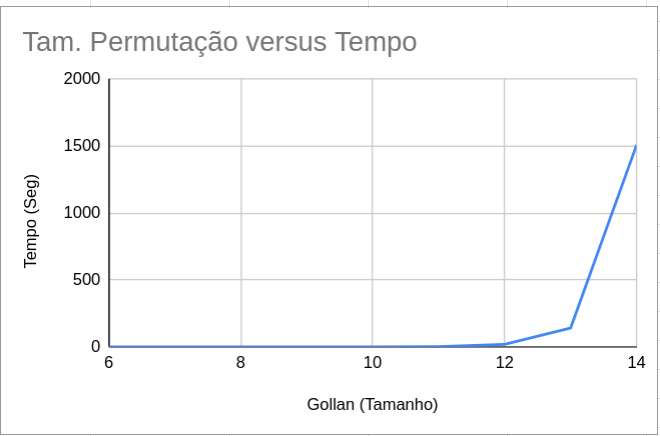
\includegraphics[width=\textwidth]{Imagens/Analises/B_PG2.png}
    \caption{\label{Grafico1}Gráfico da curva das PGs usando \textit{Branch and Bound}.}
  \end{minipage}
\end{figure}
    
\subsection{Permutações aleatórias}

A figura \ref{Grafico2} apresenta o gráfico de nossas análises utilizando PRs como entrada do algoritmo exato. Os resultados obtidos foram calculados a partir da média de 20 instâncias de teste e o intervalo do número de elementos das permutações foi de 9 elementos até 21 elementos. A partir de 21 elementos o tempo de execução dos testes ultrapassaria um limite de 6,5 horas que estipulamos e, por isso, não prosseguimos com testes maiores. A curva do gráfico esboça o comportamento do algoritmo exato e, assim como no experimento anterior, podemos inferir que estendendo este gráfico, seu tempo de execução se comportaria como uma função exponencial no tamanho da entrada.

\begin{figure}[H]
  \centering
  \begin{minipage}[b]{0.5\textwidth}
    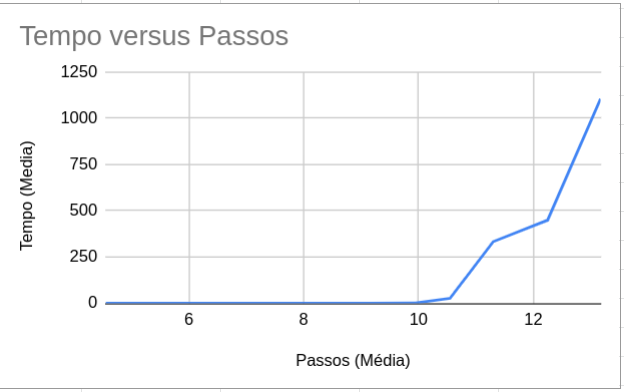
\includegraphics[width=\textwidth]{Imagens/Analises/B_PR2.png}
    \caption{\label{Grafico2}Gráfico da curva das análises usando PR como entrada para o algoritmo BnB.}
  \end{minipage}
\end{figure}

\subsection{Permutações geradas por reversões aleatórias}

A figura \ref{Grafico3} apresenta o gráfico de nossas análises referentes a PGRs como entrada do algoritmo BnB utilizando permutações de tamanho fixo de 30 elementos que são embaralhadas aplicando de 4 a 16 reversões, com incrementos de 1 em 1 para cada instância. Os resultados foram obtidos a partir de uma média de 20 testes. Podemos visualizar que ao longo do crescimento da quantidade de reversões de embaralhamento, a média da quantidade de reversões para ordenação também se mantém crescente, mas começa a se distanciar da curva de embaralhamento. Nossas estimativas são que, se pudéssemos estender estes testes, esse distanciamento seria mais evidente. Optamos pelo limite de 16 reversões, já que para prosseguir com um número maior gastaríamos um tempo superior a 5,5 horas, que foi nosso teto estipulado para cada conjunto destas análises.

\begin{figure}[H]
  \centering
  \begin{minipage}[b]{0.5\textwidth}
    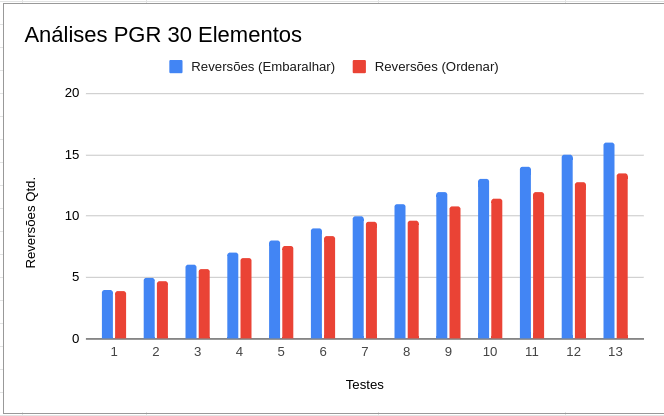
\includegraphics[width=\textwidth]{Imagens/Analises/B_PGR3.png}
    \caption{\label{Grafico3}Gráfico  de barras comparativas entre reversões usando o algoritmo \textit{Branch and bound}.}
  \end{minipage}
\end{figure}

\section{Experimentos com algoritmo \textit{Greedy}}

\subsection{Permutações de Gollan}

A figura \ref{Grafico4}, apresenta o gráfico de nossos experimentos utilizando PGs como entrada para o algoritmo \textit{Greedy}, com a quantidade de elementos da PG em um intervalo entre 10 e 495 elementos, com uma variação de 5 elementos incrementados a cada conjunto de testes, com os resultados obtidos a partir de uma média de 100 testes. É interessante observar que na curva de crescimento do tempo, um pico é apresentado a cada 10 elementos, comportamento este que podemos atribuir ao fato das PGs serem um tipo especial de permutação. 

\begin{figure}[H]
  \centering
  \begin{minipage}[t]{0.5\textwidth}
    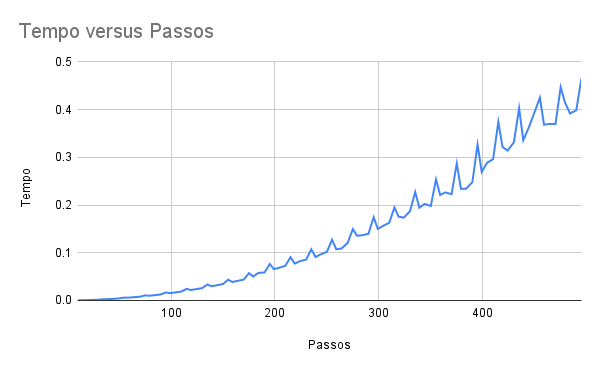
\includegraphics[width=\textwidth]{Imagens/Analises/G_PG2.png}
    \caption{\label{Grafico4} Gráfico da curva de PG como entrada do algoritmo \textit{Greedy}.}
  \end{minipage}
\end{figure}
    
\subsection{Permutações aleatórias}
    
A próxima análise representada na figura \ref{Grafico5} é referente aos experimentos utilizando PRs como entrada do algoritmo. Este conjunto de testes gerou as permutações mais extensas, demonstrando crescimento contínuo do tempo de execução, mas com alguns picos na média do tempo de execução em relação à média de passos de ordenação. As análises foram feitas utilizando permutações em um intervalo de 250 a 7750 elementos, com uma variação de 250 elementos incrementados a cada teste, com os resultados obtidos a partir de uma média de 100 testes.

\begin{figure}[H]
  \centering
  \begin{minipage}[t]{0.6\textwidth}
    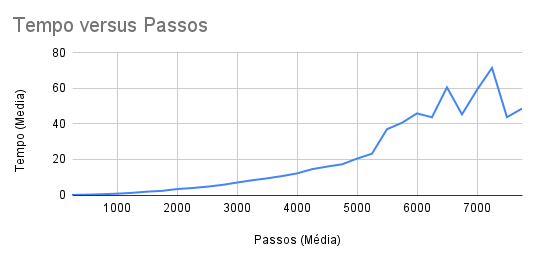
\includegraphics[width=\textwidth]{Imagens/Analises/G_PR2.png}
    \caption{\label{Grafico5} Gráfico da curva de PR como entradas do algoritmo \textit{Greedy}.}
  \end{minipage}
\end{figure}
    
\subsection{Permutações geradas por reversões aleatórias}
    
A figura \ref{Grafico6} mostra o gráfico de nossos testes sobre PGRs como entrada do algoritmo \textit{Greedy}. Os resultados foram calculados a partir da média de 100 testes com permutações de tamanho fixo de 100 elementos, com a a quantidade de reversões de embaralhamento variando de 1 à 200, incrementadas em 5 a cada teste. Verificamos um comportamento através da curva do gráfico que a medida que aumentamos a quantidade de reversões de embaralhamento, a quantidade de reversões para ordenação também cresce. Porém, a partir de um determinado ponto, a curva achata e a média da quantidade de reversões necessárias para ordenação se mantém. Este comportamento se dá pelo fato de que dentro de permutações de tamanho fixo (ou seja, que não variam), não é possível torná-las mais difíceis de se ordenar indeterminadamente apenas embaralhando-as ainda mais. Há um limite para isso e quando esse limite é alcançado, a quantidade de reversões necessárias para se ordenar a permutação torna-se independente da quantidade de reversões de embaralhamento (veja a Propriedade \ref{prop4}). O limite que encontramos neste cenário de testes está entre 70 e 75 reversões de embaralhamento. 

\begin{figure}[H]
  \centering
  \begin{minipage}[t]{0.8\textwidth}
    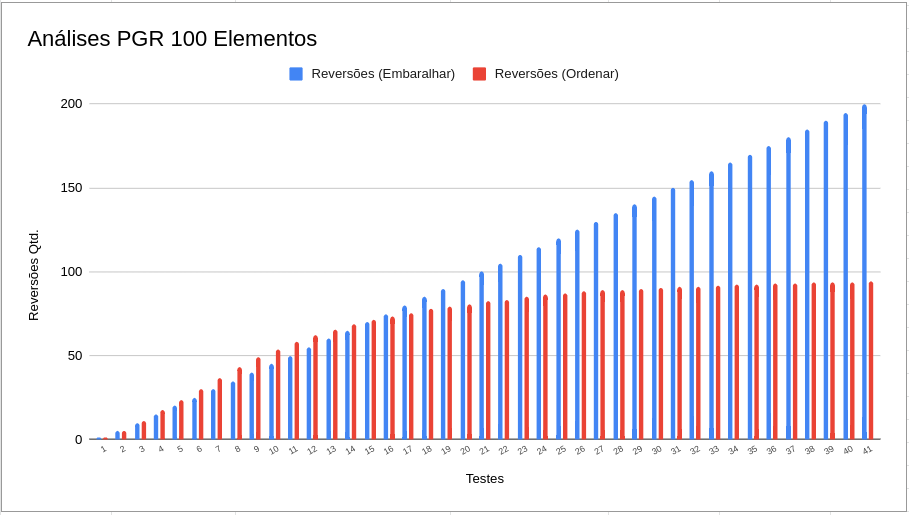
\includegraphics[width=\textwidth]{Imagens/Analises/G_PGR2.png}
    \caption{\label{Grafico6} Gráfico de  barras comparativas de reversões usando PGR como entrada do algoritmo \textit{Greedy}.}
  \end{minipage}
\end{figure}


\section{\textit{Greedy vs.~Branch and Bound}}


Nesta última análise temos um comparativo dos dois algoritmos que implementamos utilizando PGRs como entrada. Utilizamos permutações de tamanho fixo de 30 elementos e variamos a quantidade de reversões de embaralhamento num intervalo de 4 à 16 reversões, com os resultados obtidos a partir de uma média de 20 testes. Na figura \ref{Grafico7} podemos visualizar que ambas as curvas dos algoritmos acompanham o crescimento da curva de embaralhamento. Porém, a curva de crescimento do algoritmo exato (linha amarela) se mantém abaixo da curva de crescimento principal (linha azul), demonstrando que consome em média uma quantidade de passos inferior em relação à quantidade de passos do algoritmo de aproximação, um comportamento que é esperado.

\begin{figure}[H]
  \centering
  \begin{minipage}[t]{0.6\textwidth}
    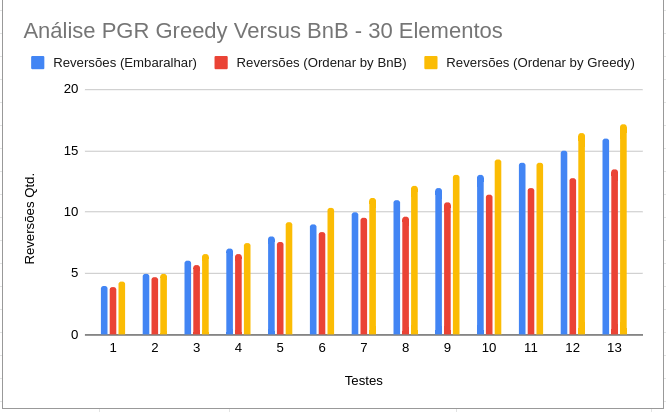
\includegraphics[width=\textwidth]{Imagens/Analises/BG_PGR.png}
    \caption{\label{Grafico7} Gráfico comparativo entre as soluções dos algoritmos \textit{Greedy} e \textit{branch and Bound}.}
  \end{minipage}
\end{figure}
    
Mantivemos um intervalo pequeno na quantidade de reversões, pois dado que o desempenho do algoritmo exato não é bom, há complicações para solucionar instâncias maiores devido ao tempo gasto para ordenar as permutações. Visto isso, descartamos do gráfico informações relativas ao tempo e focamos apenas na quantidade média de reversões necessárias para ordenar as permutações. Pressupomos também que estendendo este experimento teríamos o achatamento das curvas vermelha e amarela, pois como explicado na Propriedade \ref{prop4}, existe um limite do quanto se pode dificultar o processo de ordenação por reversões de uma permutação. 

% \FV{Olhe o rótulo na linha acima (??): lema3 não existe.}

\end{chapter}
\chapter{Conclusão}
\label{cap:conclusao}

    Quando iniciamos o projeto, tínhamos o objetivo de seguir os estudos em \cite{kececioglu1995exact}, estudar a base  teórica necessária para entender o problema de ordenação por reversões e modelar experimentos utilizando os algoritmos \textit{Greedy} e \textit{Branch and Bound} em cenários específicos a fim de descobrir as vantagens e desvantagens dos algoritmos e suas variações. Para os experimentos que fizemos, utilizar três modelagens de permutações foi fundamental para explorar mais possibilidades. Partindo do que fizemos foi possível notar um desempenho melhor do algoritmo \textit{Greedy} na maior parte dos cenários, o que no primeiro momento parece destoar dos resultados teóricos, mas compreensível pois existem fatores que tornam isso possível. Estes fatores estão ligados inicialmente com a maneira que operamos as remoções nas listas de candidatos do \textit{Branch and Bound}. Sabemos que nossos algoritmos limitantes não são os com melhor desempenho e isso impacta diretamente na quantidade de candidatos a serem percorrido, tornando o algoritmo exato mais lento. Dessa forma, nossa proposta inicial que foi de compreender a bagagem teórica do problema e executar experimentos que demonstrassem as soluções propostas pelo autor foi cumprida. Em nosso ultimo teste de comparação entre os algoritmos onde utilizamos PGRs e nivelamos o tamanho das entradas podemos ver resultados mais precisos por parte do algoritmo exato, tendência que cresce a medida que o tamanho da permutação aumenta assim como esperávamos. 
    
    Para trabalhos futuros visamos aumentar as variações de limitantes superior e inferior para o algoritmo exato, analisar os tempos de execução e com isso gerar testes com entradas maiores e mais robustas. Em nosso período de trabalho nos deparamos com uma ferramenta chamada Gurobi, um \textit{solver} utilizado para modelar e resolver funções lineares, estas que podem ser usadas como limitantes no algoritmo exato, assim como demonstrado por \cite{kececioglu1995exact}. Entendemos que essas funções lineares trarão um desempenho superior ao que temos hoje. Ao longo do desenvolvimento reestruturamos nossos objetivos, focando apenas em versões mais simples dos algoritmos, pois entendemos que seria necessário um tempo maior para nos aprofundarmos nas particularidades de cada um deles, para assim conseguir propor mudanças e melhorias.








\addcontentsline{toc}{chapter}{Referências bibliográficas}
\nocite{*}
\bibliographystyle{abbrv}
\bibliography{referencias}
\chapter{Anexos}
\appendix
\section{ANEXO I - Dados dos Experimentos.}
\url{https://docs.google.com/spreadsheets/d/1cjAI1FdGTZ12SGoAfeGNXyB5Z9SkDUBa8lEqiBPSlfA/edit?usp=sharing}

\addcontentsline{toc}{chapter}{Anexos}
\end{document}
